\chapter{Basic Set Theory and Interval Notation}

You are given either interval notation, set-builder notation, or a graph. Write each of the following in its other 2 forms. 
\begin{enumerate}
\setlength\itemsep{10pt}
    \item $(-5, 8]$
    \item $\{x|x \leq 1\}$
    \item
    \raisebox{-8pt}{
    \begin{tikzpicture}
    \draw [->] (-2,0) node [below, yshift=-4pt] {$-3$} -- (2,0);
    \draw [fill=black] (-2,0) circle [radius=2.5pt];
    \end{tikzpicture}}
    \item $\{x | x \neq 4, 11\}$
    \item
    \raisebox{-8pt}{
    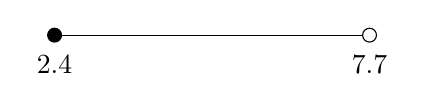
\begin{tikzpicture}
        \draw (-2,0) node [below, yshift=-4pt] {$2.4$} -- (2,0) node [below, yshift=-4pt] {$7.7$};
        \draw [fill=black] (-2,0) circle [radius=2.5pt];
        \draw [fill=white] (2,0) circle [radius=2.5pt];
    \end{tikzpicture}}
    \item $(9, \infty)$
\setcounter{Review}{\value{enumi}}
\end{enumerate}

Write each using interval notation and graph on a number line.
\begin{enumerate}
\setcounter{enumi}{\value{Review}}
\item $\{x | x \geq 2\}$
\item $\{x |x < -8\}$
\item $\{x |x \neq 3\}$
\item $\{x | x \neq -2, 5\}$
\setcounter{Review}{\value{enumi}}
\end{enumerate}

You are given the graph of an interval. Write the interval and set-builder notation for it.
\begin{enumerate}
\setcounter{enumi}{\value{Review}}
\item \raisebox{-10pt}{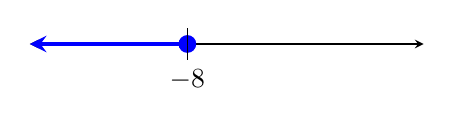
\begin{tikzpicture}[>=stealth]
    \draw[<->] (-2.5,0) -- (2.5,0);
    \filldraw[color=blue] (-0.5,0) circle [radius=3pt];
    \draw (-0.5,0.2) -- (-0.5,-0.2) node [below] {$-8$};
    \draw[color=blue,ultra thick, ->] (-0.5,0) -- (-2.5,0);
    \end{tikzpicture}}

\item \raisebox{-10pt}{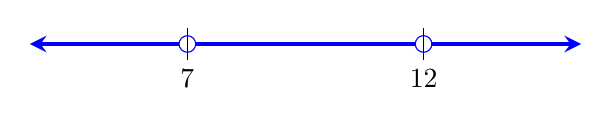
\begin{tikzpicture}[>=stealth]
    \draw[<->, color=blue, ultra thick] (-3.5,0) -- (3.5,0);
    \draw[color=blue, fill=white] (-1.5,0) circle [radius=3pt];
    \draw[color=blue, fill=white] (1.5,0) circle [radius=3pt];
    \draw (-1.5,0.2) -- (-1.5,-0.2) node [below] {$7$};
    \draw (1.5,0.2) -- (1.5,-0.2) node [below] {$12$};
    \end{tikzpicture}}
    
\item \raisebox{-10pt}{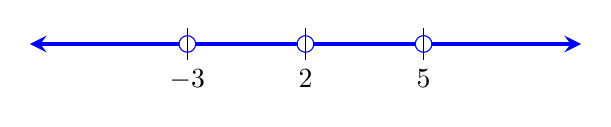
\begin{tikzpicture}[>=stealth]
    \draw[<->, color=blue, ultra thick] (-3.5,0) -- (3.5,0);
    \draw[color=blue, fill=white] (-1.5,0) circle [radius=3pt];
    \draw[color=blue, fill=white] (1.5,0) circle [radius=3pt];
    \draw[color=blue, fill=white] (0,0) circle [radius=3pt];
    \draw (-1.5,0.2) -- (-1.5,-0.2) node [below] {$-3$};
    \draw (0,0.2) -- (0,-0.2) node [below] {$2$};
    \draw (1.5,0.2) -- (1.5,-0.2) node [below] {$5$};
    \end{tikzpicture}}
\end{enumerate}

\newpage

\section{Answer Key}

\begin{enumerate}
\setlength\itemsep{10pt}
	\item $\{x | -5 < x \leq 8\}$	\newline\\
	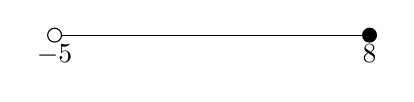
\begin{tikzpicture}
	\draw (-2,0) node [below] {$-5$} -- (2,0) node [below] {$8$};
	\draw [fill=white] (-2,0) circle [radius = 2.5pt];
	\draw [fill=black] (2,0) circle [radius = 2.5pt];
	\end{tikzpicture}
	
	\item $(-\infty, 1]$ \newline\\
	\begin{tikzpicture}
	\draw [<-] (-2,0) -- (2,0) node [below] {1};
	\draw [fill=black] (2,0) circle [radius=2.5pt];
	\end{tikzpicture}
	
	\item $[-3, \infty)$ \quad $\{x | x \geq -3 \}$
	
	\item $(-\infty, 4) \cup (4, 11) \cup (11, \infty)$ \newline\\
	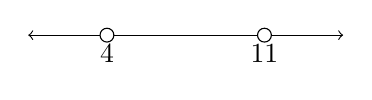
\begin{tikzpicture}
	\draw[<->] (-2,0) -- (2,0);
	\draw[fill=white] (-1,0) circle [radius=2.5pt];
	\draw[fill=white] (1,0) circle [radius=2.5pt];
	\node at (-1,0) [below] {4};
	\node at (1,0) [below] {11};
	\end{tikzpicture}
	
	\item $[2.4, 7.7)$ \quad $\{x | 2.4 \leq x < 7.7\}$
	
	\item $\{x | x > 9\}$ \newline\\
	\begin{tikzpicture}
	\draw[->] (-2,0) -- (2,0);
	\draw[fill=white] (-2,0) circle [radius=2.5pt];
	\node at (-2,0) [below] {9};
	\end{tikzpicture}

	\item $[2, \infty)$ \newline\\
	\begin{tikzpicture}
	\draw[->] (-2,0) -- (2,0);
	\draw[fill=black] (-2,0) circle [radius=2.5pt];
	\node at (-2,0) [below] {2};
	\end{tikzpicture}
	
	\item $(-\infty, -8)$ \newline\\
	\begin{tikzpicture}
	\draw[<-] (-2,0) -- (2,0);
	\draw[fill=white] (2,0) circle [radius=2.5pt];
	\node at (2,0) [below] {$-8$};
	\end{tikzpicture}
	
	\item $(-\infty, 3) \cup (3, \infty)$ \newline\\
	\begin{tikzpicture}
	\draw[<->] (-2,0) -- (2,0);
	\draw[fill=white] (0,0) circle [radius=2.5pt];
	\node at (0,0) [below] {3};
	\end{tikzpicture}
	
	\item $(\infty, -2) \cup (-2,5) \cup (5,\infty)$ \newline\\
	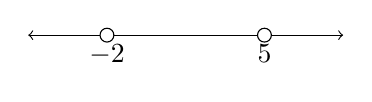
\begin{tikzpicture}
	\draw[<->] (-2,0) -- (2,0);
	\draw[fill=white] (-1,0) circle [radius=2.5pt];
	\draw[fill=white] (1,0) circle [radius=2.5pt];
	\node at (-1,0) [below] {$-2$};
	\node at (1,0) [below] {5};	
	\end{tikzpicture}
	
	\item $(-\infty, -8]$ \quad $\{ x | x \leq -8 \}$
    \item $(-\infty,7) \cup (7,12) \cup (12, \infty)$ \quad $\{ x | x \neq 7, 12 \}$
    \item $(-\infty,-3) \cup (-3,2) \cup (2, 5) \cup (5, \infty)$ \quad $\{ x | x \neq -3, 2, 5 \}$
\end{enumerate}


